\documentclass{../cours}
\usepackage{hyperref}
\title{Entraînement : listes chaînées}

\begin{document}
\maketitle

Les solutions peuvent être rédigées en \textbf{pseudo-code, python, C, C++ ou Java}. La syntaxe du langage n'a pas d'importance tant que celle-ci reste \textbf{cohérente} et \textbf{compréhensible}. (Dans les exemples, les solutions sont données en pseudo-code).

\textbf{Grille d'évaluation}

\vspace{0.5cm}

\begin{tabular}{|l|p{12cm}|}
\hline
A (20) & \small{L’algorithme répond au problème posé de façon claire et exhaustive.} \\ \hline
B (16) &\small{Le principe général de l'algorithme est le bon. Cependant, il y a une ou deux erreurs / oublis sur les cas particuliers ou les conditions d'arrêts et vérification de pointeurs nuls. Il peut y avoir des petites erreurs dans la manipulation de la liste (erreur de nom, confusion cellule / valeur)} \\ \hline
C (11) & \small{Le principe général de l'algorithme est le bon mais il y de nombreuses erreurs ou oublis de cas particuliers.}\\ \hline
D (8) &\small{Le principe général de l’algorithme ne permet pas de répondre au problème, cependant les opérations de manipulation sur la liste chaînée sont écrites correctement.} \\ \hline
E (1) & \small{L’algorithme est faux ou inexistant et la manipulation de la liste n'est pas correcte.} \\ \hline
\end{tabular}



\begin{exercice}
Une \textbf{file} est une structure de données "First In, First out" : on fait sortir les éléments dans l'ordre dans lequel ils sont arrivés. Elle accepte deux opérations \textbf{enfile} qui rajoute un élément et \textbf{defile} qui supprime l'élément le plus ancien.

Exemple, si l'on part d'une file vide \texttt{F} :

\begin{lstlisting}
enfile(F,2)
enfile(F,1)
enfile(F,3)
enfile(F,4)
Affiche defile(F)
Affiche defile(F)
Affiche defile(F)
Affiche defile(F)
\end{lstlisting}

affiche $2134$.

Et 

\begin{lstlisting}
enfile(F,2)
enfile(F,1)
Affiche defile(F)
enfile(F,3)
enfile(F,4)
Affiche defile(F)
enfile(F,5)
Affiche defile(F)
Affiche defile(F)
Affiche defile(F)
\end{lstlisting}

affiche $21345$.

On propose d'implanter une File en utilisant une structure de liste chaînée. Cependant, contrairement à d'habitude, on va maintenir \textbf{deux pointeurs} : un sur la tête de liste et un sur le dernier élément de la liste. 

\begin{lstlisting}
Structure Cellule:
    Entier valeur
    Cellule suivante

Structure File:
    Cellule premiere
    Cellule derniere
\end{lstlisting}

On enfile en fin de liste et on défile en début de liste.

Exemple illustré.

\begin{tabular}{cccc}
Liste vide
&
Enfile 2
&
Enfile 4
&
Defile
\\
\scalebox{.8}{
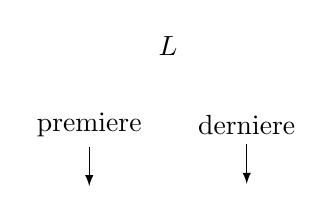
\begin{tikzpicture}[>=latex]
\node(L) at (1,0){$L$};
\node(Prem) at (0,-1){premiere};
\node(Dern) at (2,-1){derniere};

\draw (Prem.south) edge[->] ++(0,-.5);
\draw (Dern.south) edge[->] ++(0,-.5);
\end{tikzpicture}
}
&
\scalebox{.8}{
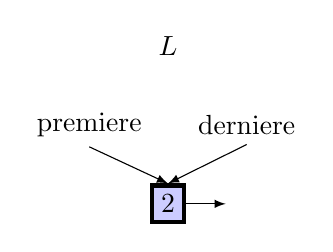
\begin{tikzpicture}[>=latex]
\node(L) at (1,0){$L$};
\node(Prem) at (0,-1){premiere};
\node(Dern) at (2,-1){derniere};

\node(T1)[draw, ultra thick, fill=blue!20, rectangle] at (1,-2) {2};

\draw (Prem.south) edge[->] (T1.north);
\draw (Dern.south) edge[->] (T1.north);
\draw (T1.east) edge[->] ++(.5,0);
\end{tikzpicture}
}
&
\scalebox{.8}{
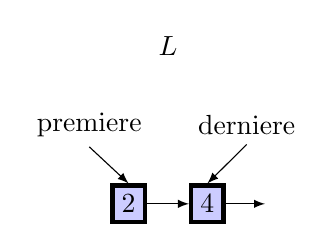
\begin{tikzpicture}[>=latex]
\node(L) at (1,0){$L$};
\node(Prem) at (0,-1){premiere};
\node(Dern) at (2,-1){derniere};

\node(T1)[draw, ultra thick, fill=blue!20, rectangle] at (0.5,-2) {2};
\node(T2)[draw, ultra thick, fill=blue!20, rectangle] at (1.5,-2) {4};

\draw (Prem.south) edge[->] (T1.north);
\draw (Dern.south) edge[->] (T2.north);
\draw (T1.east) edge[->] (T2.west);
\draw (T2.east) edge[->] ++(.5,0);
\end{tikzpicture}
}
&
\scalebox{.8}{
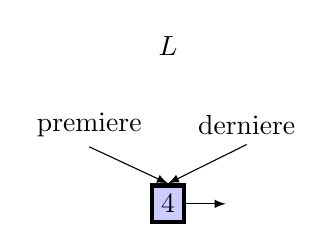
\begin{tikzpicture}[>=latex]
\node(L) at (1,0){$L$};
\node(Prem) at (0,-1){premiere};
\node(Dern) at (2,-1){derniere};

\node(T1)[draw, ultra thick, fill=blue!20, rectangle] at (1,-2) {4};

\draw (Prem.south) edge[->] (T1.north);
\draw (Dern.south) edge[->] (T1.north);
\draw (T1.east) edge[->] ++(.5,0);
\end{tikzpicture}
}
\\
\end{tabular}

Implantez les fonctions \texttt{Enfile(File F, Entier a)} (pas de valeur de retour) et \texttt{Defile(File F)} (renvoie un entier). On supposera
que l'appel \texttt{Cellule(a)} permet de créer une cellule de valeur $a$.


\textbf{Solution}

\begin{lstlisting}
Enfile
Input : File F, Entier a
Procédé :
    d <- F.derniere
    n <- Cellule(a) 
    Si d != None:
        d.suivante <- n
        F.derniere <- n
    Sinon:
        F.premiere <- n
        F.derniere <- n
        
Defile
Input : File F
Output : un entier
Procédé :
    p <- F.premiere
    Si p = None:
        Erreur
    Sinon
        v <- p.valeur
        F.premiere <- p.suivante
        Si F.premiere = None:
            F.derniere <- None
        Retourner v
\end{lstlisting}

\end{exercice}


\end{document}